\newpage
\subsection{Problems \& Exercises}

\begin{problem}
If $A \subset B \subset \mathbb{R} \Rightarrow \  \sup{A} \leq \sup{B} \wedge \ \inf{A} \geq \inf{B}$
\end{problem}

\begin{solution}
\begin{enumerate}[label=\roman*)]
\item Since $\sup{B}$ is an upper bound of $B: \forall b \in B: b \leq \sup{B}$

Since $A \subset B, \forall a \in A$ also belongs to $B \rightarrow \forall a \in A: a \leq \sup{B}$.

Therefore, $\sup{B}:$ upper bound of $A$. Finally, since $\sup{A} \in A \rightarrow \sup{A} \leq \sup{B}$ as well.
$$
\Rightarrow \sup{A} \leq \sup{B}.
$$

\item Since $\inf{B}$ is a lower bound of $B: \forall b \in B: \inf{B} \leq b$

Since $A \subset B, \forall a \in A$ also belongs to $B \rightarrow \forall a \in A: \inf{B} \leq a$.

Therefore, $\inf{B}:$ lower bound of $A$. Finally, since $\inf{A} \in A \rightarrow \inf{B} \leq \inf{A}$ as well.
$$
\Rightarrow \inf{A} \geq \inf{B}.
$$
\end{enumerate}
\end{solution}

\begin{problem}
Let $X, Y \subset \mathbb{R}$ be non empty sets, such that $x \leq y, \ \forall x \in X, \forall y \in Y $\\
Then, proof the following hold: $X$ is bounded above, $Y$ is bounded below, and $\sup{X} \leq \inf{Y}$
\end{problem}

\begin{solution}
\begin{enumerate}[label=\roman*)]
	\item Since $Y$ is non-empty, $\exists y \in Y$. Then $\forall x \in X: x \leq y$
	$\rightarrow y$ is an upper bound of $X$, so $X$ is bounded above.

	\item Since $X$ is non-empty, $\exists x \in X$. Similarly $\forall y \in Y: x \leq y$
	$\rightarrow x$ is a lower bound of $Y$, so $Y$ is bounded below.

	\item Since $Y$ is bounded below and $X$ is bounded above: $\exists \inf{Y} \land \sup{X}$ so that:
	\begin{align*}
	\forall x \in X,\ \forall y \in Y: x \leq y
	\rightarrow \forall x \in X&: \left(\forall y \in Y: x \leq y\right)\\
	\rightarrow \forall x \in X&: x \text{ is a lower bound of } Y\\
	\rightarrow \forall x \in X&: x \leq \inf{Y}
	\end{align*}

	Thus, $\inf{Y}$ is an upper bound of $X$.

	By the definition of $\sup{X}$ being the least upper bound, any other upper bound will be greater:

	$$\Rightarrow \sup{X} \leq \inf{Y}.$$
\end{enumerate}
\end{solution}

\begin{problem}\label{prob:dedekind-2}
Let $X, Y \subset \mathbb{R}$ be non empty sets, such that
$x \leq y, \ \forall x \in X, \forall y \in Y$, and suppose that
$X \cup Y = \mathbb{R}$. Prove that $\sup{X} = \inf{Y}.$
\end{problem}

\begin{solution}
From the previous result, we have: $\sup{X} \leq \inf{Y}$.
Now, let's assume that $\sup{X} < \inf{Y}$ strictly, and try to reach the absurd. Intuition tells me that the idea is to expect items between $X$ and $Y$, and to prove that this would violate the initial conditions.

\begin{center}
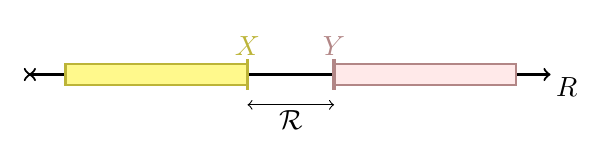
\begin{tikzpicture}[scale=.55]

    % Number line
    \draw[thick,->] (-6,0) -- (6,0);
    \draw[thick,<->] (-6,0) -- (-6.05,0); % left arrow tip

    % X region (yellow)
    \filldraw[
        fill=yellow!45,
        draw=yellow!70!black,
        thick
    ] (-5.2,-0.25) rectangle (-1,0.25);

    % Y region (pink)
    \filldraw[
        fill=pink!35,
        draw=pink!70!black,
        thick
    ] (1,-0.25) rectangle (5.2,0.25);

    % Boundary markers
    \draw[very thick,yellow!70!black] (-1,-0.35) -- (-1,0.35);
    \draw[very thick,pink!70!black] (1,-0.35) -- (1,0.35);

    % Labels
    \node[yellow!70!black] at (-1,0.65) {$X$};
    \node[pink!70!black] at (1,0.65) {$Y$};

    % Gap label
    \draw[<->] (-1,-0.7) -- (1,-0.7);
    \node at (0,-1.05) {$\mathcal{R}$};

    % Real numbers label
    \node[right] at (5.9,-0.3) {$\mathbb{R}$};

\end{tikzpicture}
\end{center}


Assuming $\sup{X} < \inf{Y}:$
\begin{align*}
\exists r \in \mathbb{R}: \sup{X} < r &\wedge r < \inf{Y} \\
\rightarrow \mathcal{R} := \{r \in \mathbb{R} / \sup{X} < r &\wedge r < \inf{Y}\} \neq \O \\
\rightarrow r \not\in X &\land r \not\in Y \\
\rightarrow r \not\in X &\cup Y \\
\rightarrow r \not\in \ \mathbb{R}& \ (\rightarrow\leftarrow)
\end{align*}

$$\therefore \sup{X} = \inf{Y}.$$
\end{solution}

\begin{problem}
\textit{Dedekind's Theorem}: Let $X, Y \subset \mathbb{R}$ be non empty sets, such that
$x \leq y, \ \forall x \in X, \forall y \in Y$, and suppose that
$X \cup Y = \mathbb{R}$. Then either $X$ has a maximal element, or $Y$ has a minimal element.
\end{problem}

\begin{solution}
Assuming $X$ is not bounded above: 
\begin{align*}
\exists \ x' \in X / \sup{X} < x' \\
\text{Since } \sup{X} = \inf{Y} \rightarrow \inf{Y} < x' \\
\text{Then } \exists \ y = \inf{Y} \in Y : y < x' \ (\rightarrow\leftarrow)
\end{align*}

Similarly, assuming $Y$ is not bounded below:
\begin{align*}
\exists \ y' \in Y / y' < \inf{Y} \\
\text{Since } \sup{X} = \inf{Y} \rightarrow y' < \sup{X} \\
\text{Then } \exists \ x = \sup{X} \in X : y' < x \ (\rightarrow\leftarrow)
\end{align*}

$$\Rightarrow X \text{ has a maximal element, or } Y \text{ has a minimal element.}$$
\end{solution}

\begin{problem}
Let $A, B \subset \mathbb{R}$, and sets defined:

\begin{itemize}
\item $A + B = \{a + b, a \in A, b \in B\}$
\item $A . B = \{a . b, a \in A, b \in B\}$
\end{itemize}

Determine if the following is true:

\begin{enumerate}[label=\roman*)]
\item $\sup{(A + B)} = \sup{A} + \sup{B}$
\item $\sup{(A . B)} = \sup{A} . \sup{B}$
\end{enumerate}
\end{problem}

\begin{solution}
\begin{enumerate}[label=\roman*)]
	\item $\forall a \in A, b \in B \rightarrow a \leq \sup{A} \wedge b \leq \sup{B}$

	Adding up both inequalities:
	\begin{align*}
	a + b \leq \sup{A} + &\sup{B}, \ \forall a \in A, b \in B \\
	\Rightarrow \sup{A} + \sup{B} &\text{ is upper bound of } A + B
	\end{align*}

	To show that $\sup{A} + \sup{B}$ is the least upper bound of $A+B$, it is sufficient to show that:
	$$
	\forall \epsilon > 0,\ \exists a+b \in A+B:
	\sup{A} + \sup{B} - \epsilon < a+b \leq \sup{A} + \sup{B}.
	$$

	Let $\epsilon > 0$ be arbitrary. Since $\epsilon/2 > 0$, by the characterization of $\sup{A}$ (\cref{th:sup-characterization}):
	$$
	\exists a \in A:
	\sup{A} - \frac{\epsilon}{2} < a \leq \sup{A}.
	$$

	Similarly, by the characterization of $\sup{B}$:
	$$
	\exists b \in B:
	\sup{B} - \frac{\epsilon}{2} < b \leq \sup{B}.
	$$

	Adding both inequalities:
	\begin{align*}
	\sup{A} + \sup{B} - \frac{\epsilon}{2} - \frac{\epsilon}{2}
	&< a+b \leq \sup{A} + \sup{B} \\
	\Rightarrow \sup{A} + \sup{B} - \epsilon
	&< a+b \leq \sup{A} + \sup{B} \\
	\Rightarrow \sup{A} + \sup{B}&: \text{least upper bound of } A+B \\
	\therefore \sup{(A+B)} &= \sup{A} + \sup{B}.
	\end{align*}

	\item By counter-example, let $A = \{1,2\}$ and $B = \{-3,-4\}$. Then:
	\begin{align*}
	A.B &= \{-3,-4,-6,-8\} \\
	\sup{(A.B)} &= -3 \neq (2.-3) = \sup{A}.\sup{B}. (\rightarrow\leftarrow)
	\end{align*}
\end{enumerate}
\end{solution}

\begin{problem}
Let $-A$ be the set of numbers of the form -a, where $a \in A \subset \mathbb{R}$.

Show that $\sup{(-A)} = -\inf{A}$.
\end{problem}

\begin{solution}
Having $\sup{(-A)} := \{-a' \in -A / \forall -a \in A: -a \leq -a' \}$
\begin{align*}
\forall -a \in A: -a \leq \sup{(-A)} \\
\rightarrow -(-a) \geq -\sup{(-A)} \\
\rightarrow -sup(-A) \leq a \\
\rightarrow -sup(-A) : \text{lower bound of } A
\end{align*}

Additionally, for $-A$ we have by the supremum definition:
\begin{align*}
\forall \epsilon > 0, &\exists x \in -A: \sup{(-A)} - \epsilon < x \leq \sup{(-A)}\\
(\text{mul.} -1)&: -\sup{(-A)} + \epsilon > -x \geq -\sup{(-A)}, -x \in A\\
(\text{fixing ineq. side})&: -\sup{(-A)} \leq -x < -\sup{(-A)} + \epsilon \\
\Rightarrow -sup{(-A)}&: \text{greatest lower bound of } A \\
\end{align*}

Finally:
\begin{align*}
-sup(-A) = inf(A) \\
\therefore sup(-A) = -\inf(A)
\end{align*}

\end{solution}

\begin{problem}
Let $A$, $B$, and $C$ be sets such that $A \subset C$, $B \subset C$, $A \setminus B \neq \O$, and $B \setminus A \neq \O$. We introduce a partial ordering into this triple of sets. Exhibit the maximal and minimal elements of the set $\{A,B,C\}$.
\end{problem}

\begin{solution}
This is the setup that the problem proposes:
\begin{figure}[H]
\centering
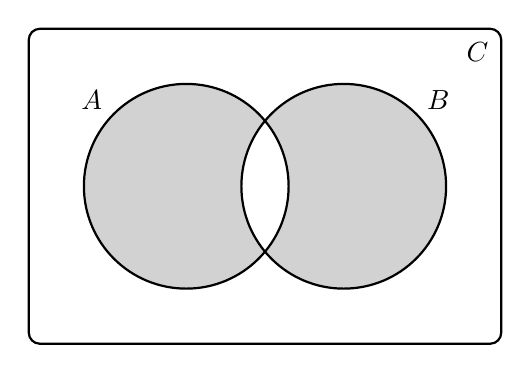
\begin{tikzpicture}

% Outer set C
\draw[thick, rounded corners] (-3,-2) rectangle (3,2);
\node at (2.7,1.7) {$C$};

% Shade A \ B
\begin{scope}
\clip (-1,0) circle (1.3cm);
\fill[gray!35] (-3,-2) rectangle (3,2);
\clip (1,0) circle (1.3cm);
\fill[white] (-3,-2) rectangle (3,2);
\end{scope}

% Shade B \ A
\begin{scope}
\clip (1,0) circle (1.3cm);
\fill[gray!35] (-3,-2) rectangle (3,2);
\clip (-1,0) circle (1.3cm);
\fill[white] (-3,-2) rectangle (3,2);
\end{scope}

% Sets A and B
\draw[thick] (-1,0) circle (1.3cm);
\draw[thick] (1,0) circle (1.3cm);

% Labels
\node at (-2.2,1.1) {$A$};
\node at (2.2,1.1) {$B$};

\end{tikzpicture}
\end{figure}

Where $A \backslash B \land B \backslash A$ are not empty. Then for set $\{A, B, C\}$:

\begin{align*}
A \subset C \land B \subset C \rightarrow A \subset B \subset C \\
\rightarrow \text{max}_{\subset}\{A, B, C\} = C \\
\end{align*}

Now, since $A \not\subset B \land B \not\subset A$:
\begin{align*}
\rightarrow \text{min}_{\subset}\{A, B, C\} \text{ is not unique.}
\end{align*}

Both $A$ and $B$ are minimal elements (sets) but none of them is the \textit{least}.
\end{solution}

\begin{problem}
Show that, just like the set $\mathbb{Q}$ of rational numbers, the set $\mathbb{Q}(\sqrt{n})$ of numbers of the form $a+b\sqrt{n}$, where $a,b \in \mathbb{Q}$ and $n$ is a fixed natural number that is not the square of any integer, is an ordered set satisfying the principle of Archimedes but not the axiom of completeness.
\end{problem}

\begin{solution}
Considering that $a, b \in \mathbb{Q}$ and that $\mathbb{Q}$ is an Archimedean (Ordered Field), we can conveniently say:
$$\exists N_a, N_b \in \mathbb{N}: |a| < N_A \land |b| < N_B$$
And since $n \in \mathbb{N}$ is a fixed number, it also satisfies:
$$\sqrt{n} < n + 1$$
Correctly adding and multiplying these three inequalities:

\begin{align*}
|a| &< N_A \\
|b| &< N_B \\
\sqrt{n} &< n + 1 \\
\rightarrow |a| + |b|\sqrt{n} &< N_A + N_B (n + 1)
\end{align*}

On the left side, we can consider $|a| + |b|\sqrt{n} = |a| + |b.\sqrt{n}|$. Then, using the triangle inequality:
\begin{align*}
|a + b.\sqrt{n}| \leq |a| + |b\sqrt{n}| = |a| + |b|\sqrt{n}
\rightarrow |a + b\sqrt{n}| < N_A + N_B (n + 1)
\end{align*}

Finally, by simple absolute value property
\begin{align*}
a + b\sqrt{n} \leq |a + b\sqrt{n}|
\end{align*}

Now, let $x = a + b\sqrt{n} \in \mathbb{Q}(\sqrt{n})$, and $N = N_A + N_B (n + 1) \in \mathbb{N}$:
\begin{align*}
\Rightarrow x < N, x \in &\mathbb{Q}(\sqrt{n}), N \in \mathbb{N}\\
\therefore \mathbb{Q}(\sqrt{n})&: \text{Archimedean}.
\end{align*}

Now, to prove that this is not a complete field, we need to form a subset $q \subset \mathbb{Q}(\sqrt{n})$ that somehow has its supremum in $\mathbb{R}$, but outside of $\mathbb{Q}(\sqrt{n})$. I found out myself that this could go one of two ways: the \textit{skadoodle-out-of-thin-air} answer, or the \textit{intuitively-looking-for-an-answer} answer. Of course I will do the second one, but in case this is too ugly for the sake of an arbitrary exercise, please feel free to skip (by the way, answer is $\sqrt[4]{n}$).

Now to build $q$ we could start with this rough idea:

\begin{center}
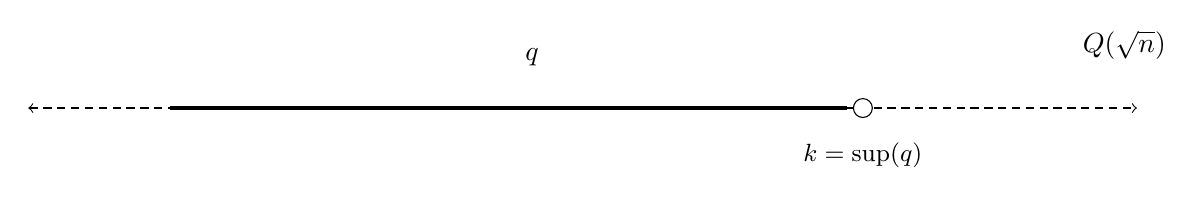
\begin{tikzpicture}[scale=4]
  \draw[<->, densely dashed] (0,2.4) -- (3.52,2.4);
  \draw[ultra thick] (0.45,2.4) -- (2.6,2.4);
  \draw[fill=white] (2.65,2.4) circle (0.03cm);
  \node[draw=none, inner sep=1.03pt] at (3.48,2.6) {$\mathbb{Q}(\sqrt{n}$)};
  \node[draw=none] at (1.6,2.56) {$q$};
  \node[draw=none, node font=\small, inner sep=1pt] at (2.65,2.25) {$k = \sup(q)$};
\end{tikzpicture}
\end{center}


Let's first assume there exists a $k$ outside of $\mathbb{Q}(\sqrt{n})$, so that our chosen set $q$ is:

$$q = \{x \in \mathbb{Q}(\sqrt{n}), x < k\}$$

By doing this, we guarantee that $k$ bounds $q$. Again, we are trying to prove that this is the supremum in such a way that we guarantee its existence outside of $\mathbb{Q}(\sqrt{n})$.

To prove that this is the lowest upper bound, let's assume the ``real'' supremum is actually a $k'$:

\begin{enumerate}[label=\roman*)]
\item Assume $\exists k': k' < k$. By density in $\mathbb{Q}:$

\begin{align*}
\exists x \in \mathbb{Q}&: k' < x < k \\
\text{Since } \mathbb{Q} \subset \mathbb{Q}(\sqrt{n}) \rightarrow \exists x \in \mathbb{Q}(\sqrt{n})&: k' < x < k. \\
\rightarrow x &\in q \\
\rightarrow k' &\text{not L.U.B of } q
\end{align*}

\end{enumerate}

And so, by showing that every number smaller than $k$ fails to be an upper bound for $q$, while $k$ itself is an upper bound, we prove that
$$k = \sup(q).$$

Now, this is just half of the proof. At the beginning we assumed that this $k$ exists, and I don't appreciate left over assumptions. The next proof is to make sure that there is at least a number that allows us to create $q$. Let's call it $\lambda$ and try to prove $\exists \lambda \in \mathbb{R}: \lambda \not\in \mathbb{Q}(\sqrt{n})$.

\begin{align*}
\lambda \not\in \mathbb{Q}(\sqrt{n}) \leftrightarrow \lambda \not= a + b\sqrt{n}
\end{align*}

My intent is to apply some sort of transformation to both sides, and get to an absurd. I tried several things ($\log$, factorial, $\exp$, etc), but the only clue I got back is that the $\sqrt{n}$ was in the way. Then I realized that, as long as I can find a $\lambda$ whose square is of the form $A+B\sqrt{n}$, I could compare coefficients and try to force an absurd.

In other words, I want
\begin{align*}
\lambda^2=A+B\sqrt{n}.
\end{align*}

The simplest choice seems to be
\begin{align*}
A=0,\qquad B=1,
\end{align*}
which gives
\begin{align*}
\lambda^2&=\sqrt{n}\\
\lambda&=\sqrt{\sqrt{n}}\\
\lambda&=\sqrt[4]{n}.
\end{align*}

Now, we still need to prove that this choice of $\lambda$ is actually outside of $\mathbb{Q}(\sqrt{n})$. So, let's assume the opposite and try to force an absurd:
$$
\sqrt[4]{n}=a+b\sqrt{n}
$$
for some $a,b\in\mathbb{Q}$.

Trying to square everything:
\begin{align*}
\sqrt{n}&=(a+b\sqrt{n})^2\\
&=a^2+b^2n+2ab\sqrt{n}\\
&=(a^2+b^2n)+(2ab)\sqrt{n}.
\end{align*}

Now, the trick is to realize that both sides are written in the form $A+B\sqrt{n}$, so we can compare coefficients. Since $\sqrt{n}\notin\mathbb{Q}$, this representation is unique. Therefore:
\begin{align*}
0&=a^2+b^2n\\
1&=2ab.
\end{align*}

Now, $a^2+b^2n\geq0$ for all $a,b\in\mathbb{Q}$ and $n\in\mathbb{N}$. For it to be zero, we must have
$$
a=b=0.
$$
But then
$$
2ab=0\neq1,
$$
which is a contradiction.

Therefore,
$$
\sqrt[4]{n}\notin\mathbb{Q}(\sqrt{n}).
$$

Finally, we can define
$$
q=\{x\in\mathbb{Q}(\sqrt{n}),x<\sqrt[4]{n}\}.
$$

I have the hunch that it is possible to find other numbers besides $\sqrt[4]{n}$ that also satisfy to be an outsider supremum. I raised the same comparison for $\lambda$ to the third and fourth exponent, and could only find an absurd scenario for the latter one, making me think that these numbers live in a set like
$$
\Lambda=\{\sqrt[2k]{n},k\in\mathbb{N}\}.
$$

It would need induction to be proven, but I don't have that kind of time.
\end{solution}

\begin{problem}
Show that the set $\mathbb{Q}(x)$ of rational fractions

$$\frac{a_0+a_1x+\cdots+a_mx^m}{b_0+b_1x+\cdots+b_nx^n}$$

with coefficients in $\mathbb{Q}$ or $\mathbb{R}$ becomes an ordered field, but not an Archimedean ordered field, when the order relation $R_{m,n} \succ 0$ is defined to mean $a_m b_n>0$ and the usual arithmetic operations are introduced.
\end{problem}

\begin{solution}
First let's address the order defined as:
$$R_{m,n} \succ 0 \leftrightarrow a_mb_n > 0$$
To prove order, we must check the set's behavior over trichotomy, and closure over addition and multiplication (\cref{th:ordered-field-criterion}). We must also make sure that the order is well-defined, since the same rational function can have more than one representation.

\begin{enumerate}[label=\roman*)]
\item \textbf{Well-definedness:}

Suppose that the same rational function can be written in two different ways:
$$\frac{P(x)}{Q(x)}=\frac{R(x)}{S(x)}.$$
Then
$$P(x)S(x)=R(x)Q(x).$$

Let the leading coefficients of $P,Q,R,S$ be respectively $a_m,b_n,c_p,d_q$. Comparing the leading coefficients on both sides gives:
$$a_md_q=c_pb_n.$$

Therefore, the two representations have the same sign under the proposed order. Hence, whether $R_{m,n}\succ0$ or $R_{m,n}\prec0$ does not depend on the particular representation chosen.

\item \textbf{Trichotomy:}

Since the given order ``$\succ$'' subtly misses defining the equality, and we need to check if a given element could be either greater, less than or \textbf{equal} to zero, we need to consider the case where the numerator is the zero polynomial.

If the numerator is zero, then:
$$R_{m,n}=0.$$

Otherwise, the leading coefficients $a_m,b_n$ are both non-zero, and therefore exactly one of $a_mb_n>0$ or $a_mb_n<0$ holds. We have:
\begin{align*}
&a_mb_n > 0 \leftrightarrow R_{m,n} \succ 0 \\
&a_mb_n < 0 \leftrightarrow -a_mb_n > 0 \leftrightarrow -R_{m,n} \succ 0 \leftrightarrow 0 \succ R_{m,n}.
\end{align*}

Therefore, exactly one of $$R_{m,n}=0,\qquad R_{m,n}\succ0,\qquad 0\succ R_{m,n}$$
holds, satisfying trichotomy.

\item \textbf{Closure over $\oplus$:}

Solving for any pair of $R_{m,n} \oplus R_{p,q}$, $R_{m,n}, R_{p,q} \succ 0$:
\begin{align*}
R_{m,n} \oplus R_{p,q}
&= \frac{a_0 + \dots + a_mx^m}{b_0 + \dots + b_nx^n}
+ \frac{c_0 + \dots + c_px^p}{d_0 + \dots + d_qx^q}\\
&= \frac{(a_md_qx^{m+q})+(c_pb_nx^{p+n}) + \mathbb{S}_1}
{b_nd_qx^{n+q} + \mathbb{S}_2}.
\end{align*}

We will just consider the terms containing the leading degree of both sides of the fraction. Since the order just depends on these, we can skip evaluating the rest by indicating a left over expression added up as $\mathbb{S}_{1,2}$. Then, we have two possibilities for the coefficient of the leading degree: $a_md_q$ or $c_pb_n$.

If the degrees $m+q$ and $p+n$ are different, the term with the larger degree leads. If they are equal, the two leading terms are added together. In this case, we need to make sure that they do not cancel.

Noticing as well that since both $R_{m,n}, R_{p,q} \succ 0 \rightarrow a_mb_n > 0 \land c_pd_q > 0$, we evaluate:
\begin{itemize}
	\item If $a_md_q$ leads:
	$$a_md_qb_nd_q = a_mb_n d_q^2 > 0.$$

	\item If $c_pb_n$ leads:
	$$c_pb_nb_nd_q = c_pd_q b_n^2 > 0.$$
\end{itemize}

Therefore, in either case, the leading coefficient of the numerator has the same sign as the leading coefficient of the denominator. If $m+q=p+n$, then both leading coefficients have the same sign, so they cannot cancel and their sum preserves that sign.

Meaning that either way, we preserve the order on addition:
$$\Rightarrow R_{m,n} \oplus R_{p,q} \succ 0.$$

\item \textbf{Closure over $\otimes$:}

\begin{align*}
R_{m,n} \otimes R_{p,q}
&= \frac{a_0 + \dots + a_mx^m}{b_0 + \dots + b_nx^n}
\cdot \frac{c_0 + \dots + c_px^p}{d_0 + \dots + d_qx^q}\\
&= \frac{(a_mc_px^{m+p}) + \mathbb{S}_1}
{b_nd_qx^{n+q} + \mathbb{S}_2}.
\end{align*}

Under the same condition $a_mb_n > 0 \land c_pd_q > 0$, we get that
$$a_mc_pb_nd_q=(a_mb_n)(c_pd_q)>0.$$

Therefore:
$$\Rightarrow R_{m,n} \otimes R_{p,q} \succ 0.$$

\end{enumerate}

The usual arithmetic operations on rational functions give the usual field structure, and the properties above show that the proposed order is compatible with addition and multiplication. Therefore, $\mathbb{Q}(x)$ is an ordered field.

Now, to prove that $\mathbb{Q}(x)$ is not an Archimedean ordered field, we need to prove that there is at least one element in $\mathbb{Q}(x)$ that is larger than every element of $\mathbb{N}$.

Let $k\in\mathbb{N}$. Consider $x-k\in\mathbb{Q}(x)$:
$$x-k=\frac{x-k}{1}.$$

The leading coefficient of the numerator is $1$, and the leading coefficient of the denominator is also $1$, so:
$$1\cdot1>0 \Rightarrow x-k\succ0.$$

Therefore:
\begin{align*}
&x-k\succ0 \Rightarrow x\succ k,\qquad \forall k\in\mathbb{N}\\
&\Rightarrow \exists x\in\mathbb{Q}(x): x>k,\qquad \forall k\in\mathbb{N}\\
&\therefore \mathbb{Q}(x)\text{ is not Archimedean}.
\end{align*}
\end{solution}
